\section{Software prototyping}
\subsection{Embedded development environment}

Software shoud take care of the motor control, IMU output readings and remote control, this could create complications, as essentially they would interrupt each other. A way of multitasking should be introduced.
"An RTOS (Real-Time Operating System) is a software component that lets you rapidly switch between different running sections of your code. Think of it as having several loop() functions in an Arduino sketch where they all run at the same time." \cite{Joe2019}

After research, the list was narrowed to two top condenders – FreeRTOS and Zephyr. Both solutions are open source, widely used and support the Microcontroller board we have chosen. \cite{Lemberg}
According to 2018 IoT Developer Survey \cite{IOT}, FreeRTOS is one of the most popular OS used and while Zephyr only received a 2.8 \% rating in 2018, it is often described as one of the fastest growing RTOS and in 2022 has become the largest open-source RTOS project by the number of commits and developers. (See Figure~\ref{fig:iot_os})
\begin{figure}[H]
    \centering
    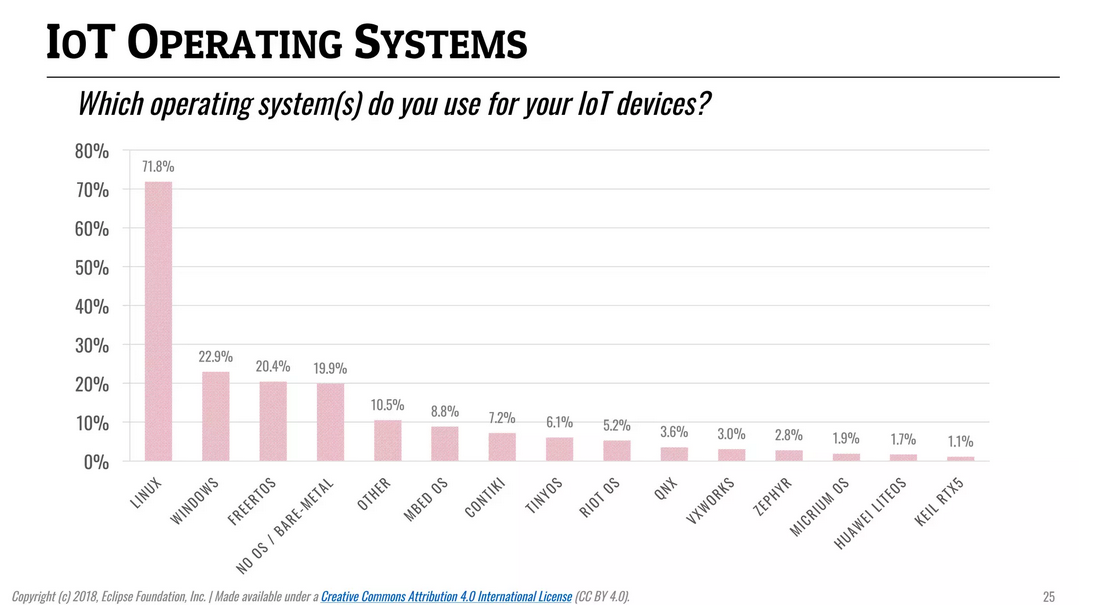
\includegraphics[scale = 0.5]{pictures/iot_os.PNG}
    \caption{IoT Developer Survey 2018 results}
    \label{fig:iot_os}
\end{figure}

To decide between the RTOS choice, a pros and cons table was created and evaluated. \cite{Comparison} (See Table~\ref{table.rtos})

\begin{table}[H]
      \makegapedcells
  \setlist[itemize]{font=\color{black},
                    nosep,
                    leftmargin=*,
                    after=\vspace*{-\baselineskip}}
      \setlength{\tabcolsep}{3pt}
  \begin{tabularx}{\linewidth}{|>{\RaggedRight}p{25mm}|*{2}{I |}}
      \hline
  RTOS
      &   \mcl{Advantages}    &   \mcl{Disadvantages}        \\
      \hline
  FreeRTOS 
      &   \item Suitable for begginers
          \item Open source – online comunity support available 
          \item Libraries for Seeed XIAO Sense available
          \item Constantly improved
          \item Fast code execution
          \item Low memory consuption
          &   \item Not event-driven (scheduler will only be called once in a certain period of time)
              \item Less flexible
              \\
      \hline
  ZephyrRTOS
      &   \item Open source – online comunity support available
          \item Libraries for Seeed XIAO Sense available
          \item Constantly improved
          \item Designed to ensure energy efficiency
          \item Highly configurable
          \item Event-driven
          \item Kernel can create additional system threads
          \item Possible to exclude multithreading
          \item Additional debugging features
          \item Supported by Nordic Semiconductor
          &   \item More difficult to set-up
              \item Potentially complicated to use with no experience
              \\
      \hline

\end{tabularx}
\caption{Comparison between ZephyrRTOS and FreeRTOS}
\label{table.rtos}
\end{table}

It was evaluated, that overall FreeRTOS seems to be a better established more simple solution to be used in case of no experience, whereas Zephyr offers more flexibility and is a fast growing popular solution well suited for our application and would be a worthwile investment to build our skillset for future projects. \cite{Industry}

PlatformIO is an open-source extension of Visual studio code, which supports hundreds of boards with different frameworks. \cite{Platform} Seeed XIAO nRF52840 is not natively suported. Seeed made library for Arduino IDE, which supports Arduino and Mbed framework, that was implemented through Github to PlatformIO and allows non-problematic implementation.
The XIAO has library in the Zephyr Github repository, but the PlatformIO does not use most recent version. The version of Zephyr itself is altered in PlatformIO and therefore does not work even after corssreferencing with other boards already implemented in PlatformIO, such as Seeeduino (as a reference for the formfactor) or nRF52840 DK (as a reference for the chip).
The PlatformIO does not have inbuild serial USB communication, which results in inability to reprogram the board through the VS Code and need to go through bootloader first. This poses inconvinience, which can be avoided by use of a Arduino IDE, therefore if route of MBed or Arduino framework is chosen, Arduino IDE should be chosen. If the route of Zephyr is chosen, SDK by nordic semi is the optimal route, because event though it also does not have serial USB, it uses barebone Zephyr.

Opon further research, the Seeeduino XIAO nRF52840 Sense uses the nRF52840 microcontroler, so looking to Nordic Semiconductor nRF Connect SDK for development, which uses a RTOS called ZephyrRTOS.
Additionally, the SDK provides useful tools for development, such as build, flashing and debugging actions. \cite{nRF}


Seeed XIAO nRF52840 is not natively suported on on nRF Connect SDK, but as ZephyrRTOS supports it. \cite{docsZephyr}

There is a caviat around this, we can fetch profiles from GitHub of the current version of Zephyr via \path{Zephyr/boards/arm/xiao_ble} at main branch \cite{gitZephyr} and import the needed files into the SDK version of Zephyr we have.
In our case the path of the files would be in \path{~\ncs\v2.3.0-rc1\zephyr\boards\arm} .
After doing so, following the steps in the DevAcademy, nRF Connect SDK Fundamentals, Lesson 1 can be followed for setup. Then a blinky application can be created, and built via nRF Connect.
After a build of the application is created, a files for flashing will be created in the "build" subdirectory of the application.
To flash the Seeed XIAO nRF52840 Sense chip, entering a bootloader is needed, as it ships with the Adafruit nRF52 Bootloader, which supports UF2 flashing. \cite{docsZephyr}
Further more, a zephyr.ut2 file can be found in the "build" subdirectory of the application, after building the application, as we have done.
To access the bootloader, connect the Seeed XIAO to a PC.
Now to enter and flash an application, the reset button on the Seeed board should be clicked two times in quick succession, this will propmt the memory of the Seeed board on your PC.
Now find the previously mentioned zephyr.ut2 and drag it in to the memory of the Seeed board, and this will flash the board with the new application.

A issue accured when trying to test the "Hello World" application, when connecting to serial monitor no output is given.
After further investigation, it was noticed that the Seeed documentation, mentiones no debugging interface, hence no USB serial exists.
To solve the issue, an application called "console", from \path{zephyr/samples/subsys/usb/console} was cloned, in order to test a virtual USB serial connection, with the use of CDC ACM UART. \cite{gitZephyr}
After building and flashing, results were achieved. (See Figure~\ref{fig:serial})

\begin{figure}[H]
    \centering
    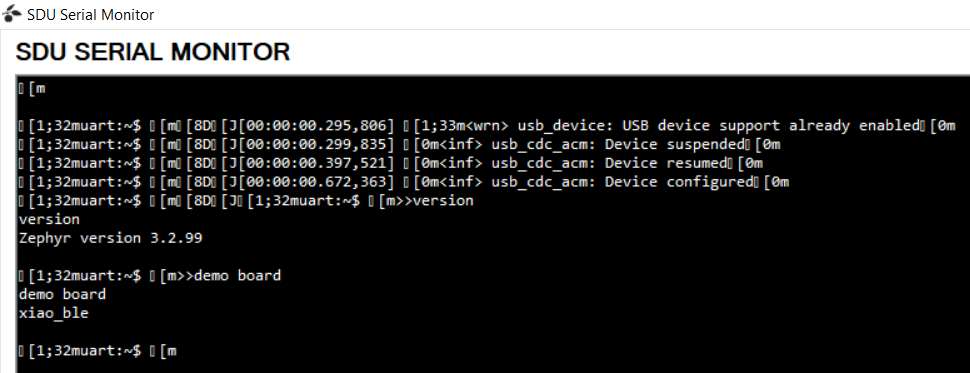
\includegraphics[scale = 0.7]{pictures/serial_monitor.png}
    \caption{Serial output of the XIAO MCU}
    \label{fig:serial}
\end{figure}

Another issue that arose was debugging. The Seeed XIAO nRF52840 Sense does not have any sort of built in debugging tools. \cite{wikiSeeed}
One can use a J-link debugging tool, but a caviet was found, which was GDB stub, which Zephyr supports, this would save budget. \cite{docsZephyr}

After achieving a succesful development cycle, it was conducted, that the use of ZephyrRTOS is possible with our current setup.
After further consultation with the supervisors, it was conducted, that the writers of the project have no skills in RTOS, more specifically in threading, and with the guidence of Davi, it was concluded, that acquiring such skills would be outside the scope of the project, as the main focus is control engineering.